\chapter[Our Framework at Work on the iTrust SWaT System]{Our Framework at Work: Reverse Engineering of the iTrust SWaT System}
\label{application}
\linenumbers

\lettrine{I}{n this} chapter, our main objective is to apply the framework and methodology introduced in Chapter \ref{chap:proposal} to the case study of the iTrust SWaT system, as illustrated in Chapter \ref{casestudy}. The purpose of this analysis is to assess the effectiveness and potential of the proposed framework within the context of a system that closely replicates a real-world water treatment plant, albeit on a smaller scale.

\bigskip
Due to the complexity of the system and the limited space available in this thesis, we will not conduct a comprehensive analysis and reverse engineering of the entire system. Instead, we will focus on specific parts for analysis. We leave it to the reader or those interested in utilizing the proposed methodology and framework to complete the analysis, should they choose to do so.\newline
By focusing on selective components and leaving room for further exploration, we strike a balance between providing valuable insights and acknowledging the potential for additional research. This approach empowers the reader and interested individuals to explore the iTrust SWaT system further and leverage the proposed methodology and framework for a more comprehensive analysis.

\section{Preliminary Operations}
\label{sec:6_preliminar_operations}
Prior to beginning the actual analysis, several preliminary manual operations need to be conducted on the physical process dataset utilized as a case study, specifically the SWaT system dataset for the year 2015 as outlined in Section \ref{subsec:5_2015_datasets}. To simulate the data-capture process performed by Ceccato et al. using their scanning tool, the original dataset in XLSX format (proprietary to Microsoft Excel) was divided into multiple datasets in CSV format. Each of these datasets corresponds to the individual stages of the SWaT system and contains the respective registers. These resulting files were then saved in the directory specified by the \texttt{raw\_dataset\_directory} directive in the framework configuration file, \textit{config.ini}, ready to be used in the pre-processing phase.\newline
Furthermore, the headers were manually renamed by adding a prefix from \texttt{P1\_} to \texttt{P6\_} to each register's name. This prefix indicates the stages, ensuring that each register is easily identifiable and linked to its corresponding stage.

\section{Planning the Analysis Strategy}
\label{sec:6_analysis_strategy}
The complexity of the system being analyzed necessitates the adoption of a deliberate strategy for the analysis. It is not feasible to rely on trial and error or attempt every possible combination between stages. The former approach may overlook crucial relationships between PLCs or between registers, while the latter may result in excessive and unproductive efforts if the specific portion of the system being analyzed lacks significant information or relationships. \newline
A sound analysis strategy helps us focus on the important parts of the system, improving the quality of the analysis and leading to better process comprehension. By prioritizing our attention, we can gain a deeper understanding of the crucial components, resulting in more informed decision-making and a comprehensive understanding of the overall processes.

\bigskip
To define this strategy, a potential starting point could involve analyzing network traffic to determine the communication patterns and participants within the system. This can be accomplished by utilizing the techniques discussed in Section \ref{subsec:4_network_analysis} on Network Analysis. By applying the Python script described in that section to the data extracted from the network traffic dataset debated in Section \ref{par:5_2015_net_dataset}, we can generate a (simplified) network graph, as illustrated in Figure \ref{fig:6_network_SWaT}.

\begin{figure}[ht]
	\centering
	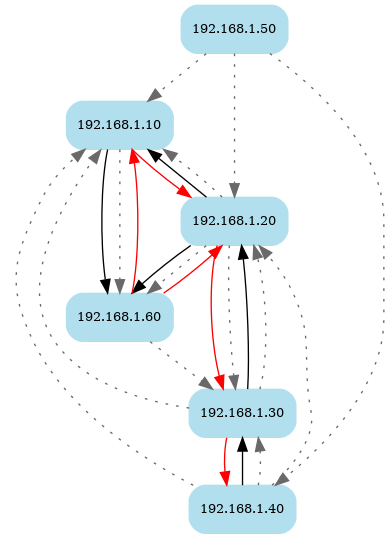
\includegraphics[scale=0.65]{chap6/network2.png}
	\caption{Simplified graph of the iTrust SWaT system network}
	\label{fig:6_network_SWaT}
\end{figure}

The graph clearly illustrates the structure of communications between the PLCs. Referring back to Table \ref{table:5_swat_ip_addresses}, which displays the IP address - PLC associations, we can observe that PLCs 1 through 4 communicate directly and sequentially with each other in a Request/Response communication pattern (represented by red and black arrows, respectively). Additionally, PLC6 communicates with both PLC1 and PLC2. On the other hand, the gray dotted arrows indicate communications for which we have knowledge of a response, but the corresponding request is unknown. For the purposes of our analysis strategy, we will not consider these communications within this context.

\bigskip
Based on our observations, the analysis strategy we will adopt involves considering sequential pairs of PLCs to effectively capture the relationships and implications between registers. Therefore, the PLC pairs we will focus on are PLC1-2, PLC2-3, and PLC3-4. 

\section{Reverse Engineering of the iTrust SWaT System}
\label{sec:6_reverse_SWaT}
Before we delve into the analysis, it is important to provide some preliminary remarks. 

\bigskip
Firstly, the analysis will be structured as a schematic analysis due to space constraints, which prevent us from presenting the extensive inferences and reasoning regarding the system in full detail. However, the general procedure of the methodology and how to reason about the data obtained from the framework have already been demonstrated through examples on the PLC1 of the SWaT system in Chapter \ref{chap:proposal}. We encourage readers to refer to those examples for a more comprehensive understanding. In this analysis, our focus will be on illustrating the conjectures and properties that arise from the analysis, utilizing tables and the outputs generated during the analysis.

\bigskip
The second premise addresses the process of defining the subsystems to be analyzed, which were obtained during the pre-processing phase, during the merge phase of the individual datasets. Apart from the projection determined by the considered PLCs, a time-based selection of the analysis period has also been performed (see Section \ref{subsubsec:4_select_subsystem}). This selection spans a duration of 20,000 seconds, which is equivalent to approximately five and a half hours or roughly five system cycles. The analysis begins at 100,000 seconds, which corresponds to approximately 27 hours from the start of the available data. This deliberate selection aims to exclude the initial transient period during which the SWaT system is initialized. We believe that this time range is more than sufficient for accurately defining the characteristics of the SWaT system components.

\bigskip
The third premise introduces some conventions regarding the PLC registers that will be utilized during the analysis. These conventions aid in identifying the nature and function of the registers. Specifically:

\begin{enumerate}
	\item Registers containing discrete values, such as binary or ternary values, are likely to represent actuators.
	
	\item Registers with continuous values are identified as measurements.
	
	\item Actuators with three states are recognized as valves, while those with two states are considered pumps.
	
	\item Sensors with a wide range between the maximum and minimum values are identified as level sensors for tanks. Sensors with a narrow range may represent other types of measurements such as flow or pressure sensors.
	
	\item Registers with a single constant value are recognized as either relative setpoints or backup actuators. The distinction is made based on the value contained in the register. Binary values or values corresponding to the states of the main actuators indicate backup actuators, while different values (e.g., 20, 40, 80, etc.) suggest the presence of relative setpoints.

	\item Registers with similar names, such as \texttt{P1\_LIT101} and \texttt{P3\_LIT301}, or \texttt{P2\_MV201} and \texttt{P3\_MV302}, indicate the same type of register, such as a valve, pump, level sensor, or other category.
\end{enumerate}

By following these conventions, it becomes easier to interpret and analyze the functionality of the PLC registers within the system.

\subsection{Reverse Engineering of PLC1 and PLC2}
\label{subsec:6_P1P2_analysis}
The initial focus of analysis will be on the pair comprising PLC1 and PLC2. Let's delve into the main features of this subsystem by examining the outcomes obtained from applying the framework to it.

\subsubsection{Pre-processing - Preliminary Analysis}
\label{subsubsec:6_P1P2_preprocessing}

Listing \ref{lst:6_preproc_P1P2} shows the outcomes obtained from automatic recognition of sensors and actuators:

\begin{lstlisting}[language=bash, numbers=left, caption=Preliminary analysis outcomes for sensors and actuators of \texttt{PLC1-2}, label=lst:6_preproc_P1P2]
	Actuators: 
	P1_MV101 [0.0, 1.0, 2.0]
	P1_P101 [1.0, 2.0]
	P2_MV201 [0.0, 1.0, 2.0]
	P2_P203 [1.0, 2.0]
	P2_P205 [1.0, 2.0]
	
	Sensors: 
	P1_FIT101 {'max_lvl': 2.7, 'min_lvl': 0.0}
	P1_LIT101 {'max_lvl': 815.1, 'min_lvl': 489.6}
	P2_AIT201 {'max_lvl': 256.5, 'min_lvl': 252.9}
	P2_AIT202 {'max_lvl': 8.4, 'min_lvl': 8.3}
	P2_AIT203 {'max_lvl': 342.8, 'min_lvl': 320.0}
	P2_FIT201 {'max_lvl': 2.5, 'min_lvl': 0.0}
	
	Hardcoded setpoints or spare actuators: 
	P1_P102 [1.0]
	P2_P201 [1.0]
	P2_P202 [1.0]
	P2_P204 [1.0]
	P2_P206 [1.0]
\end{lstlisting}

\noindent Based on the output presented in the listing, we have compiled a preliminary set of conjectures and properties for the subsystem in question. These findings are summarized in Table \ref{table:6_p1p2_actuators_1}:

{
	\small
	\begin{longtable}[l]{p{0.01\textwidth} p{0.45\textwidth} p{0.46\textwidth}}
		\hline
		\textbf{\#} & \textbf{Conjecture / Property} & \textbf{Reason} \\
		\hline
		
		1 & \texttt{P1\_LIT101}, \texttt{P1\_FIT101}, \texttt{P2\_FIT201}, \texttt{P2\_AIT201}, \texttt{P2\_AIT202}, \texttt{P2\_AIT203} are \textbf{measurements}. & Registers contain continuous numerical values.\\
		\hline
		
		2 & \texttt{P1\_LIT101} is identified as the \textbf{level sensor} specifically associated with a \textbf{tank} & Sensor has a wide range of values (minimum 489, maximum value of 815).\\
		\hline
		
		3 & \texttt{P1\_MV101}, \texttt{P1\_P101}, \texttt{P2\_MV201}, \texttt{P2\_P203} and \texttt{P2\_P205} are \textbf{actuators}. & Registers contain discrete numerical values.\\
		\hline
		
		4 & \texttt{P1\_MV101} and \texttt{P2\_MV201} assume three distinct states, represented by the values 0, 1, and 2. They can be identified as \textbf{valves}.& Obvious from the output and from point 3 of the third premise in Section \ref{sec:6_reverse_SWaT}\\
		\hline
		
		5 & \texttt{P1\_P101}, \texttt{P2\_P203} and \texttt{P2\_P205} assume two distinct states, represented by the values 1, and 2. They can be identified as \textbf{pumps}. & Obvious from the output and from point 3 of the third premise in Section \ref{sec:6_reverse_SWaT}\\
		\hline
		
		6 & \texttt{P1\_102}, \texttt{P2\_P201}, \texttt{P2\_P202}, \texttt{P2\_P204} and \texttt{P2\_P206} are \textbf{spare actuators}. & Registers contain constant numerical values.\\
		\hline 
		
		7 & A spare actuator in state 1 is considered to be \textbf{OFF}. & Assumption on the actuator states.\\
		\hline
		
		\caption{Likely measurements and actuators conjectures for PLC1-2}
		\label{table:6_p1p2_actuators_1}
	\end{longtable}
}

\bigskip
Continuing with the examination of the outcomes from the preliminary analysis, Listing \ref{lst:6_preproc_P1P2_time} shows the state durations of \texttt{P1\_MV101} and \texttt{P2\_MV201}:

\begin{lstlisting}[language=bash, numbers=left, caption=Time duration of the states of actuators MV101 and MV201 of PLC1-2, label=lst:6_preproc_P1P2_time]
	Actuator state durations:
	P1_MV101 == 0.0
	9  9  10  9  9  10  9  9  10  9
	
	P1_MV101 == 1.0
	1174  1168  1182  1160  1172
	
	P1_MV101 == 2.0
	669  3019  3012  3000  2981
	
	P2_MV201 == 0.0
	8  8  8  9  9  8  9  9  9  9
	
	P2_MV201 == 1.0
	1057  1057  1045  1038  1039
	
	P2_MV201 == 2.0
	120  3135  3144  3127  3109
\end{lstlisting}

\bigskip
\noindent Based on these data, we can derive a conjecture about the state 0 of the valves (Table \ref{table:6_p1p2_mvstate0}): 

{
	\small
	\begin{longtable}[l]{p{0.01\textwidth} p{0.45\textwidth} p{0.46\textwidth}}
		\hline
		\textbf{\#} & \textbf{Conjecture / Property} & \textbf{Reason} \\
		\hline
		
		8 & The state 0 of a valve is a \textbf{transient state}. & The duration of state 0 is only a few seconds. However, the subsequent states, have a significantly longer duration.\\
		\hline
		
	\caption{Conjecture on the state 0 of actuators}
	\label{table:6_p1p2_mvstate0}
\end{longtable}
}

\bigskip
In the analysis of actuator state changes relative to measurements, we referred to examples from Section \ref{subsubsec:4_brief_analysis} that demonstrated the behavior of \texttt{P1\_P101}. Applying the same reasoning also to \texttt{P1\_MV101} we can derive the conjectures described in Table \ref{table:6_p1p2_p101}:

{
	\small
	\begin{longtable}[l]{p{0.01\textwidth} p{0.45\textwidth} p{0.46\textwidth}}
		\hline
		\textbf{\#} & \textbf{Conjecture / Property} & \textbf{Reason} \\
		\hline
		
		9 & State 1 of the pump \texttt{P1\_P101} corresponds to the \textbf{OFF state} of the actuator; state 2 of \texttt{P1\_P101} corresponds to the \textbf{ON state} of the actuator. & Derived from Conjecture 7.\\ 
		\hline
				
		10 & The \textit{relative setpoints} of \texttt{P1\_P101} are approximately 535 (minimum) when state change to 1 and approximately 813 (maximum) when state change to 2. & Observation derived from output\\
		\hline
		
		11 & \texttt{P1\_P101} is responsible for \textbf{emptying the tank} represented by \texttt{P1\_LIT101}. & Derived from Conjecture 9 and 10 \\
		\hline
		
		12 & Pumps are responsible for \textbf{water outflow}. & Corollary to Conjecture 11\\
		\hline		
		
		13 & State 1 of the valve \texttt{P1\_MV101} corresponds to the \textbf{OFF state} of the actuator; state 2 of \texttt{P1\_MV101} corresponds to the \textbf{ON state} of the actuator. & Derived from Conjecture 7.\\
		\hline
		
		14 & The \textit{relative setpoints} of \texttt{P1\_MV101} are approximately 500 (minimum) when state change to 2 and approximately 800 (maximum) when state change to 1. & Observation derived from output\\
		\hline
		
		15 & \texttt{P1\_MV101} is responsible for \textbf{filling the tank} represented by \texttt{P1\_LIT101}. & Derived from Conjecture 13 and 14 \\
		\hline
		
		16 & Valves are responsible for \textbf{water intake}. & Corollary to Conjecture 15\\
		\hline

		\caption{Conjecture on valves and pumps}
		\label{table:6_p1p2_p101}
	\end{longtable}
}

\noindent Based on the conjecture, we can speculate that the level of the tank monitored by register \texttt{P1\_LIT101} is regulated by valve \texttt{P1\_MV101} at the inlet and valve \texttt{P1\_P101} at the outlet. However, the role of sensor \texttt{P1\_FIT101} is still uncertain, although in Section \ref{subsubsec:4_brief_analysis} we assumed it to be a flow or pressure sensor, and requires further investigation.

\bigskip
Regarding the elements controlled by PLC2, the analysis does not reveal the presence of another tank. Therefore, we cannot determine the exact role of sensors \texttt{P2\_AIT\textit{20x}} and \texttt{P2\_FIT201} at this point.\newline
However, there is a similarity observed between the relative setpoints of \texttt{P1\_P101} and those of \texttt{P2\_MV201}, \texttt{P2\_P203}, and \texttt{P2\_P205}. These registers exhibit very similar values during state changes, suggesting a potential relationship or similar control behavior between them.

\subsubsection{Graphs and Statistical Analysis}
\label{subsubsec:6_P1P2_graphs}
Figure \ref{fig:6_P1P2_graph_full} illustrates the graphical representation of the registers in PLC1-2 and their respective trends.

\begin{figure}[ht]
	\centering
	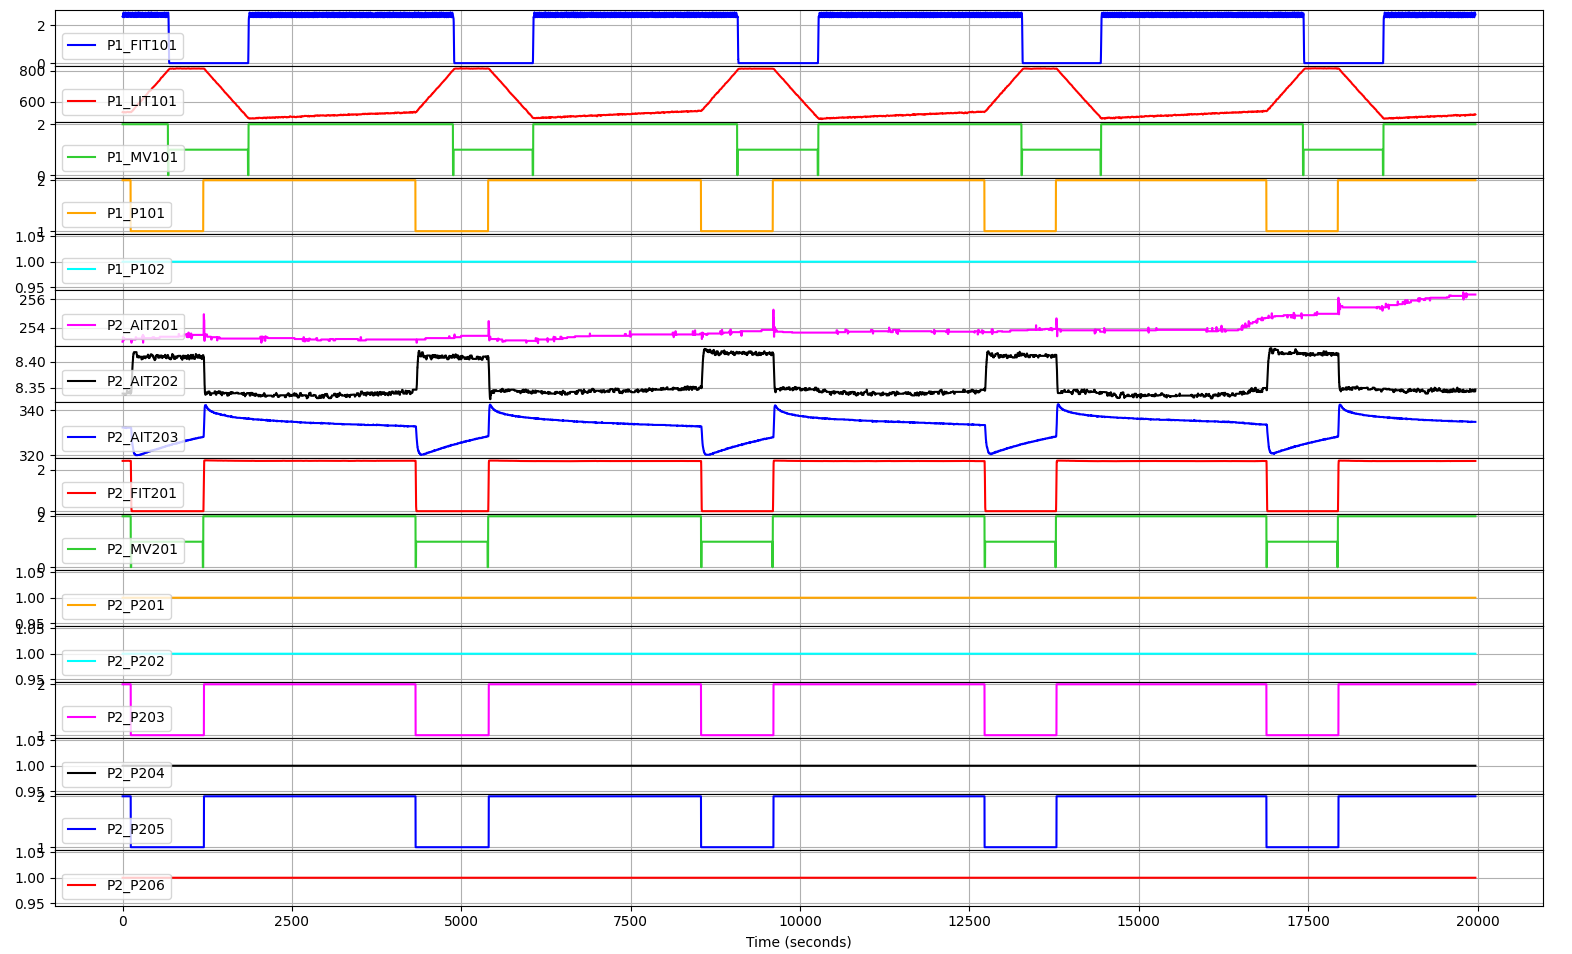
\includegraphics[scale=0.35]{chap6/P1P2_1.png}
	\caption{Chart of PLC1-2}
	\label{fig:6_P1P2_graph_full}
\end{figure}

\noindent The image provides further support for Conjecture 6 and 7: \texttt{P1\_P102}, \texttt{P2\_P201}, \texttt{P2\_P202}, \texttt{P2\_P204}, and \texttt{P2\_P206} are \textbf{backup actuators}, specifically \textbf{pumps}. These actuators consistently maintain a state of 1 and do not seem to have any significant impact on the measurements. This confirmation also supports the inference made in Conjecture 9 that state 1 of the pumps corresponds to the \textbf{OFF state}, while state 2 corresponds to the \textbf{ON state}. As a result, we can exclude these registers from further analysis.\newline 
Figure \ref{fig:6_P1P2_graph_full_nospare} provides a clearer representation of the subsystem after removing the spare actuators.

\begin{figure}[ht]
	\centering
	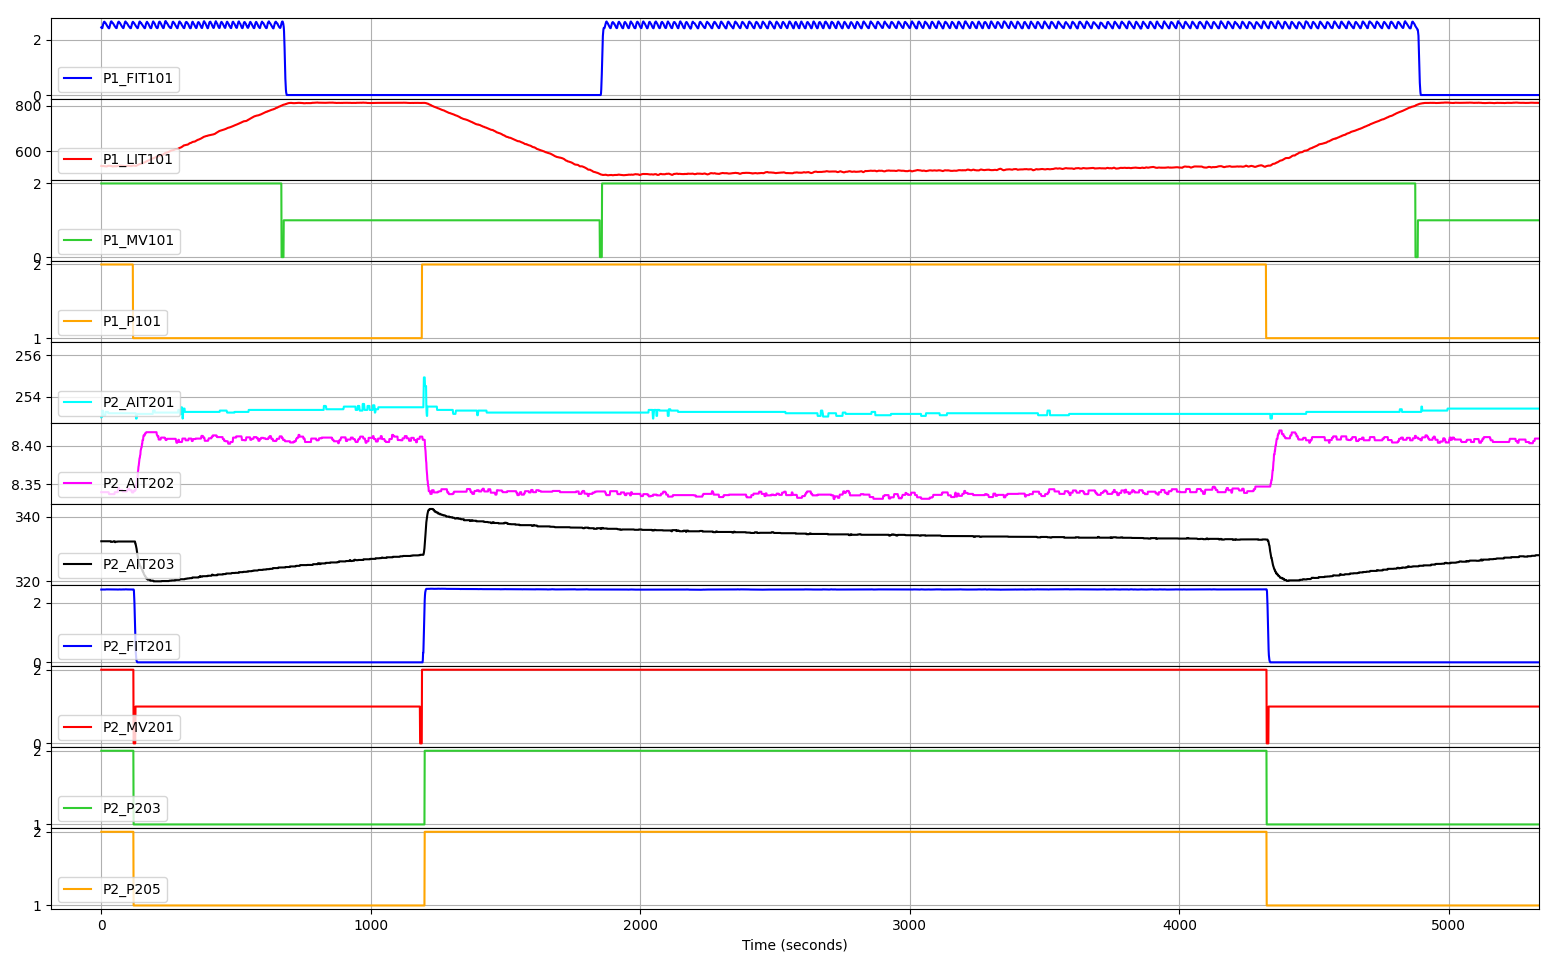
\includegraphics[scale=0.35]{chap6/P1P2_5.png}
	\caption{Chart of PLC1-2 without spare actuators (particular)}
	\label{fig:6_P1P2_graph_full_nospare}
\end{figure}

Conjecture 1 and 2, which involve the identification of the tank level sensor and measurements, are confirmed by the charts. Additionally, Conjecture 11 and 12 regarding pump behavior and Conjecture 15 and 16 regarding valve behavior in relation to the tank are also validated. Furthermore, Conjecture 8, which suggests that valves have a 0 state, is also confirmed.\newline
Looking at the plot, we can make further conjectures based on the observed trends and patterns (Table \ref{table:6_p1p2_graph_conj_1}):

{
	\small
	\begin{longtable}[l]{p{0.01\textwidth} p{0.45\textwidth} p{0.46\textwidth}}
		\hline
		\textbf{\#} & \textbf{Conjecture / Property} & \textbf{Reason} \\
		\hline
		17 & The trend of \texttt{P1\_FIT101} follows the trend of \texttt{P1\_MV101} & \texttt{P1\_FIT101} takes a value of 0 when the valve \texttt{P1\_MV101} is OFF, and positive values (> 2) when the valve is ON.\\
		\hline
		
		18 & \texttt{P1\_FIT101} is a \textbf{flow sensor} related to the inlet water flow at \texttt{P1\_LIT101}. & Corollary to Conjecture 17\\ 
		\hline
		
		19 & \texttt{P2\_FIT201} is also a likely \textbf{flow sensor}. & By analogy with \texttt{P1\_FIT101} (point 6 of the third premise in Section \ref{sec:6_reverse_SWaT})\\ 
		\hline
		
		20 & There is a correlation between the trend of \texttt{P1\_P101} and the trend of \texttt{P2\_MV201}. & Observation derived from the plot\\ 
		\hline
		
		21 & \texttt{P2\_MV201} is responsible for \textbf{filling a tank} that is \textit{not} part of this subsystem. & Sensors \texttt{P2\_AIT202} and \texttt{P2\_AIT203} do not exhibit an increasing trend when the valve is ON, and there is no apparent correspondence between the trend of the valve and the trend of \texttt{P1\_LIT101}.\\ 
		\hline
		
		22 & \texttt{P2\_AIT201} is a sensor that measures \textbf{some property of the water}. & Sensor does not show a cyclic pattern in its measurements.\\
		\hline
		
		23 & \texttt{P2\_AIT202} is a sensor that measures \textbf{some property of the water}. & Very narrow range between maximum and minimum values (point 4 of the third premise in Section \ref{sec:6_reverse_SWaT})\\
		\hline
		
		24 & The trend of \texttt{P2\_AIT202} and \texttt{P2\_AIT203} follows the trend of \texttt{P2\_P20x} pumps & Observation derived from the plot\\ 
		\hline
		
		\caption{Conjecture on the charts}
		\label{table:6_p1p2_graph_conj_1}
	\end{longtable}
}

\bigskip
Currently, the specific role of \texttt{P2\_AIT203} sensors and the correlation between \texttt{P2\_P20x} pumps and \texttt{P2\_AIT202} and \texttt{P2\_AIT203} sensors cannot be determined. These aspects require further analysis and investigation as they exhibit a cyclic pattern that seems to be associated with the behavior of the pumps.

\vfill

\subsubsection{Invariant Inference and Analysis}
\label{subsubsec:6_P1P2_invariants}

\subsubsection{Business Process Analysis}
\label{subsubsec:6_P1P2_bpa}

\subsection{Reverse Engineering of PLC2 and PLC3}
\label{subsec:6_P2P3_analysis}

\subsubsection{Pre-processing}
\label{subsubsec:6_P2P3_preprocessing}

\subsubsection{Graphs and Statistical Analysis}
\label{subsubsec:6_P2P3_graphs}

\subsubsection{Invariant Inference and Analysis}
\label{subsubsec:6_P2P3_invariants}

\subsubsection{Business Process Analysis}
\label{subsubsec:6_P2P3_bpa}

\subsection{Reverse Engineering of PLC3 and PLC4}
\label{subsec:6_P3P4_analysis}

\subsubsection{Pre-processing}
\label{subsubsec:6_P3P4_preprocessing}

\subsubsection{Graphs and Statistical Analysis}
\label{subsubsec:6_P3P4_graphs}

\subsubsection{Invariant Inference and Analysis}
\label{subsubsec:6_P3P4_invariants}

\subsubsection{Business Process Analysis}
\label{subsubsec:6_P3P4_bpa}

\vfill
\nolinenumbers